 %%%%%%%%%%%%%%%%%%%%%%%%%%%%%%%%%%%%%%%%%
% Journal Article
% LaTeX Template
% Version 1.3 (9/9/13)
%
% This template has been downloaded from:
% http://www.LaTeXTemplates.com
%
% Original author:
% Frits Wenneker (http://www.howtotex.com)
%
% License:
% CC BY-NC-SA 3.0 (http://creativecommons.org/licenses/by-nc-sa/3.0/)
%
%%%%%%%%%%%%%%%%%%%%%%%%%%%%%%%%%%%%%%%%%

%----------------------------------------------------------------------------------------
%	PACKAGES AND OTHER DOCUMENT CONFIGURATIONS
%----------------------------------------------------------------------------------------
\documentclass[twocolumn]{article}

\usepackage[french]{babel}

\usepackage[utf8]{inputenc}
\usepackage{graphicx} %pour mettre des figures dans multicol avec l'environnement figure*

%\usepackage[sc]{mathpazo} % Use the Palatino font
\usepackage[T1]{fontenc} % Use 8-bit encoding that has 256 glyphs
\linespread{1.05} % Line spacing - Palatino needs more space between lines
\usepackage{microtype} % Slightly tweak font spacing for aesthetics

\usepackage[hmarginratio=1:1,top=20mm, right=20mm]{geometry} % Document margins
\usepackage{multicol} % Used for the two-column layout of the document
\usepackage[hang, small,labelfont=bf,up,textfont=it,up]{caption} % Custom captions under/above floats in tables or figures
\usepackage{booktabs} % Horizontal rules in tables
%\usepackage{float} % Required for tables and figures in the multi-column environment - they need to be placed in specific locations with the [H] (e.g. \begin{table}[H])
\usepackage{hyperref} % For hyperlinks in the PDF

\usepackage{lettrine} % The lettrine is the first enlarged letter at the beginning of the text
\usepackage{paralist} % Used for the compactitem environment which makes bullet points with less space between them
\usepackage{bm}
\usepackage{amsfonts}
\usepackage{amsmath}
\usepackage{amssymb}

\usepackage{titlesec} % Allows customization of titles
\renewcommand\thesection{\Roman{section}} % Roman numerals for the sections
\renewcommand\thesubsection{\arabic{section}.\arabic{subsection}} % Roman numerals for subsections
\titleformat{\section}[block]{\bfseries\large\scshape\centering}{\thesection.}{1em}{} % Change the look of the section titles
\titleformat{\subsection}[block]{\bfseries\large}{\thesubsection.}{1em}{} % Change the look of the section titles

\usepackage{fancyhdr} % Headers and footers
\pagestyle{fancy} % All pages have headers and footers
\fancyhead{} % Blank out the default header
\fancyfoot{} % Blank out the default footer
\renewcommand{\headrulewidth}{0pt} %pour enlever la ligne du header
%\fancyhead[C]{titre, date, noms...	} % Custom header text
\fancyfoot[RO,RE]{\thepage} % Custom footer text
\fancyfoot[LO,LE]{A. DINSENMEYER, juillet 2017}
\renewcommand{\footrulewidth}{0.4pt} 
 
 
%agrandissement de la zone de texte
%\addtolength{\oddsidemargin}{-1cm}
%\addtolength{\evensidemargin}{-1cm}
%\addtolength{\textwidth}{2cm}
%\addtolength{\topmargin}{-0.7cm}
\addtolength{\textheight}{1cm}

\usepackage{todonotes}
\usepackage{mathtools}

%\usepackage{cite} 
\usepackage[round,authoryear,numbers]{natbib}


\usepackage{hyperref}
\hypersetup{
     colorlinks   = true,
     citecolor    = blue!90
}

\newcommand{\dd}{\partial}

%----------------------------------------------------------------------------------------
%	TITLE SECTION
%----------------------------------------------------------------------------------------

%\title{\vspace{-15mm}\fontsize{24pt}{10pt}\selectfont\textbf{Imagerie par application de la FWI à des signaux ultrasonores}} % Article title
 \title{
\centering \fontsize{18pt}{10pt}\textbf{Étude bibliographique : Méthodes de localisation de sources aéroacoustiques}
}
\author{
\large{Alice \textsc{Dinsenmeyer}}\\[2mm] % Your name %\thanks{}
%\normalsize University of California \\ % Your institution
%\normalsize \href{mailto:john@smith.com}{john@smith.com} % Your email address
\vspace{-5mm}
}
\date{}

%----------------------------------------------------------------------------------------

\begin{document}

\maketitle % Insert title

\thispagestyle{fancy} % All pages have headers and footers


%----------------------------------------------------------------------------------------
%	ARTICLE CONTENTS
%----------------------------------------------------------------------------------------

%\begin{multicols}{2} % Two-column layout throughout the main article text

Intro : localisation de sources dans le sous-sol, dans des tissus humains, dans des pièces industrielles, dans les fluides (avec ou sans écoulement, dans un espace clos ou non). La nature des sources varie.
But : caractériser quantitativement/qualitativement les sources à partir de mesures obtenue en quelques points  discrets de l'espace.

Contexte : Réduction du bruit des avions par la compréhension des bruits (40 fois plus d'énergie dans 1 kg de kérosène que dans 1 kg des meilleures batterie, après calcul de rendement, il reste un rapport 15 entre les 2).\\
Enjeu : identifier les mécanismes de génération de bruit ; 

historique :Dès 1976, pour répondre à des problématiques de compréhension des bruits de turboréacteur, \cite{billingsley_1976} réalisent des mesures simultanées à l'aide d'une antenne linéaire constituées de 14 microphones. 
Depuis, le nombre de capteur par antenne a augmenté, ainsi la gamme fréquentielle.



\todo[inline]{Pour chaque méthode : \\
-hypothèses et connaissances a priori\\
-avantages et inconvénient\\
-contexte de développement\\
-algorithme de résolution}
\todo[inline]{4 sources de problème dans la qualité de la reconstruction:\\
-bruit de mesure\\
-modèle de propagation approché\\
-modèle de source approché\\
-pb inverse mal posé : le nombre de source est souvent bien supérieur au nombre de microphones}

%sources aéros et médole de propagation en écoulement
%%===================================================
\section{Modèle de propagation et nature des sources aéroacoustiques}
%===================================================


On décrit ici les sources de bruit d'un avion à turboréacteur double flux, les méthodes de séparation des différentes contributions et les mécanismes de génération de bruits en écoulement.\\


Le bruit peut être généralement décomposé en 4 composantes : \\
-une partie tonale générée par les composantes tournantes de la machine\\
-une partie cyclostationnaire induite par les composantes tournantes de la machine\\
-le bruit machine aléatoire \\
-le bruit de fond (indépendant de la machine) (aérodynamique ?)\\


Séparer ces composantes dans le champ total mesuré permet de mieux comprendre la contribution de chaque source ou de chaque élément du réacteur, par exemple.




\subsection{Exemples de sources aéroacoustiques sur un avion}
%=============================================================

\todo[inline]{Un bref récap des sources est fait en intro de la thèse de G. Reboul et Simon B.}
\cite{Smith1989} décrit un très grand nombre de sources aéroacoustisques sur un avion. Elles peuvent être classées en 2 catégories : le bruit de moteur et le bruit aérodynamique. Le bruit aérodynamique est principalement généré par le train d'atterrissage et par les ailes. La principale source de bruit des ailes est liée aux volets à l'avant (becs de bord d'attaque) et à l'arrière. Ces volets sont des hypersustentateurs qui augmentent la portance qui génèrent localement beaucoup de bruit. Mais paradoxalement, leur présence contribuent fortement à la réduction du bruit des avions par le fait qu'ils favorisent un décollage rapide et un atterrissage à vitesse réduite.\\
Comme le montre l'image de \cite{Smith1989} \ref{smith}, les bruits du moteur sont d'origines diverses. Les moteurs doubles flux ont permis de fortement diminuer le bruit de jet, ce qui rend le bruit aérodynamique égal voire prépondérant sur le bruit de moteur en configuration d'approche (atterrissage).

\begin{figure}[!h]
 \begin{center}
  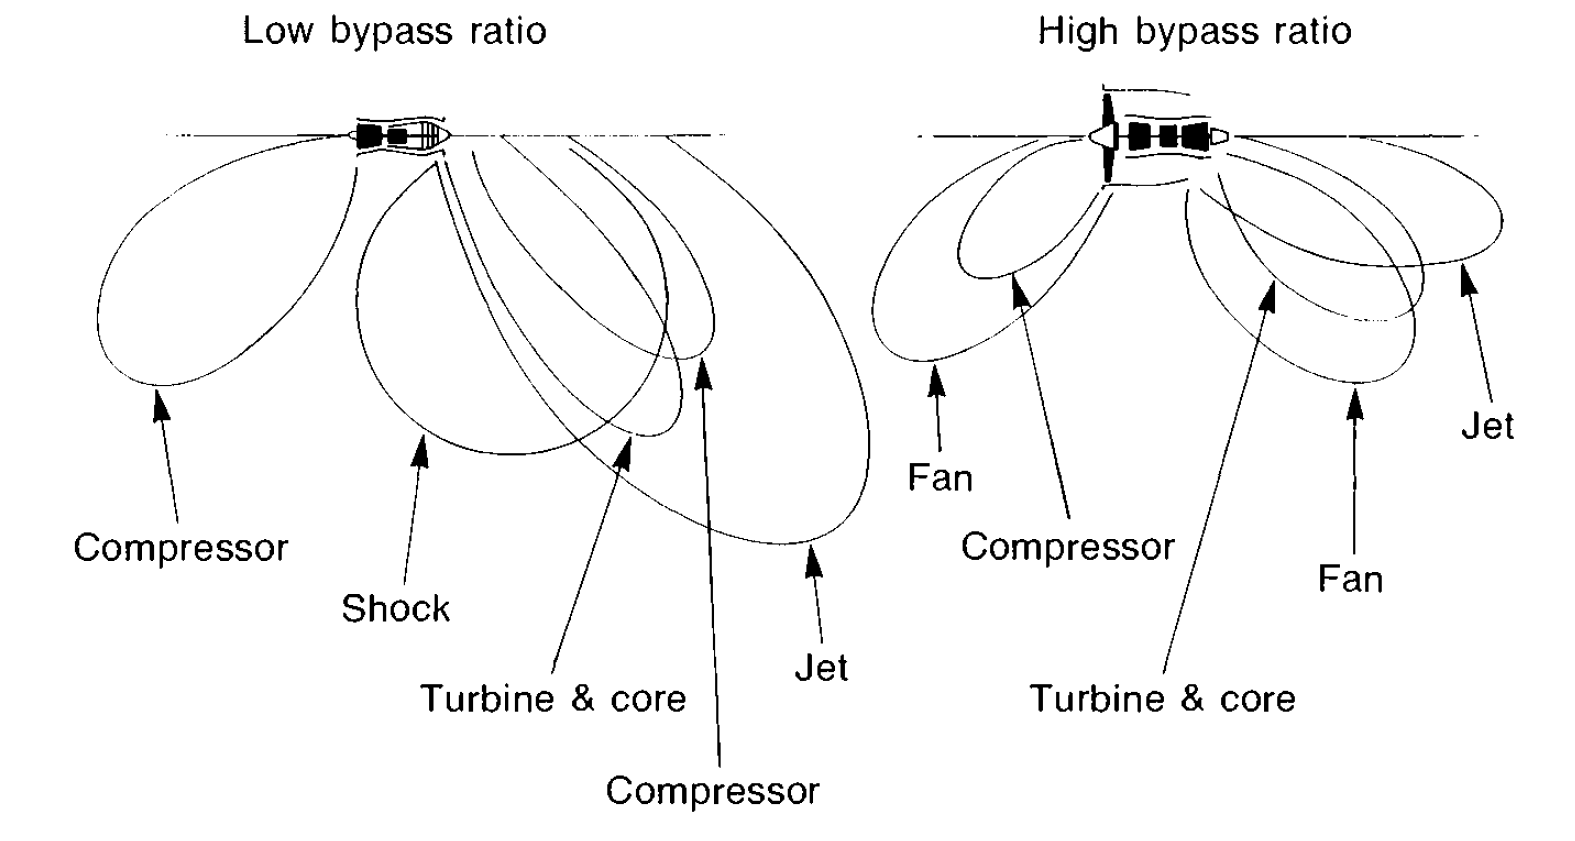
\includegraphics[width=0.5\textwidth]{img/smith_noise.png}
  \caption{Comparaison des sources de bruits d'un moteur simple flux (à gauche) et d'un moteur double flux (à droite). Image extraite de \cite{Smith1989}.\label{smith}}
 \end{center}
\end{figure}


\paragraph{Bruits tonaux}~\\
	$\bullet$ Fréquence de passage des pales (BPF : blade pass frequency) et ses harmoniques : bruit tonal, connu : $\omega = h Z \Omega$, $h=1,2,...$,  où $Z$ est le nombre de pales du rotor et $\Omega$ est sa fréquence de rotation. Les harmoniques qui apparaissent sont alors donnés par : $m=hZ-sV$, avec $m$ le numéro du mode azimutal, $V$ le nombre de pale du stator et $s=...,-1,0,1,...$\\
	$\bullet$ Bruit d'épaisseur (Blade thickness noise) : monopole, tonal. C'est le bruit généré par le déplacement du fluide autour des pales (présent à haute vitesse de rotation seulement).\\
	$\bullet$ Uniform inlet flow : peut être réduit en augmentant le nombre de pales\\

 

\paragraph{Bruits large bande}~\\
	\tbullet Flux inconstant : fluctuation stochastique de la vitesse du flux entrant génère un bruit large bande\\
	\tbullet Couche limite turbulente (TBL : Turbulent Boundary layer) : couche turbulent générée aux bords de fuite. Ce bruit peut être modélisé comme un ensemble de dipôles répartis sur la surface de l'aube.\\
	\tbullet Décollement de couche limite (Vortex shedding) : décollement de la couche limite (laminaire ou turbulente), ce qui change l'écoulement autour des pales\\
	\tbullet tip noise : bruit généré dans l'espacement entre les pales et le carter. Ce bruit augmente si l'espacement augmente. A noter que la vitesse à l'extrémité des pales étant grande, ce bruit peut être important.\\
	\tbullet Bruit de soufflante : dans les turboréacteurs double-flux principalement. Ref : thèse G. reboul\\


Bruit d'interaction rotor-stator : dominant ?\\
\todo[inline]{Compléter en lisant la thèse de Simon}

Les moteurs double flux ont permis de diminuer l'importance du bruit de jet, mais ont rajouté le bruit de soufflante.


\subsubsection{Bruit de jet}

page 86 de Smith : Description du bruit de jet\\
-small-scale Eddies (HF)\\
-large-scale Eddies (BF)\\
-mixing region\\
-shock noise\\
Sur un moteur à low-bypass-ration, le centre du jet sort à 500 m/s de la tuyère, et constitue la principale source de bruit du turbo réacteur.\\
Depuis les turboréacteurs double-flux, le jet chaud est entouré du jet froid issu de la soufflante.\\


L'enjeu est donc de séparer ces composantes pour extraire seulement le bruit induit par les sources d'intérêt.





\subsection{Physique de la Propagation acoustique en écoulement}
%=================================================================

Pour ces méthodes, on considère que la façon dont le son se propage est connue (matrice de transfert acoustique). Prendre en compte l'écoulement, sinon les sources apparaissent décalées vers l'aval (Amiet, par ex). 
Calibration de la matrice interspectrale avec et sans écoulement : ne nécessite pas de connaître la nature de l'écoulement. (S.Kroeber,K.Ehrenfried,L.Koop et A.Lauterbach, « In-flow calibration approach for improving beamforming accuracy) Mais contrainte expérimentale car coûteux en temps et surveillance des fluctuation de Temperature...\\


Pour comprendre le problème, il est nécessaire de rappeler les expression analytique de l'intensité acoustique rayonnée par un écoulement.

\subsubsection{Équations classiques de la mécanique des fluides}
\vspace{0.3cm}\paragraph{Conservation de la quantité de mouvement : Navier-Stokes}
\begin{equation}
	\frac{\dd \rho u_i}{\dd t} + \frac{\dd \rho u_i u_j}{\dd x_j} = -\frac{\dd p}{\dd x_i} + \rho g_i + \frac{\dd \tau_{ij}}{\dd x_j}
\end{equation}
\paragraph{Conservation de la masse}
\begin{equation}
 \frac{\dd \rho}{\dd t} + \frac{\dd \rho u_{i}}{\dd x_i} = 0
\end{equation}

\todo[inline]{Poursuivre après cours d'aéroacoustique}



%Nature des sources : différent niveaux, cohérent/incohérent, étendues/ponctuelles ? Hypothèses sur les sources : ondes planes/sphériques, par ex.

%Fonctions de Green en écoulement

%Spécificité de l'imagerie en écoulement turbulent

%Correction de l'écoulement : modèle d'Amiet ou modèle de Koop
%Étude de la correction à appliquer pour l'écoulement en beamforming : thèse Haddad.


%Source dipolaire/monopolaire : influence sur la méthode ?

%Nature du bruit de fond ?

%\todo[inline]{Prise en compte des réflexions sur le jet, interaction non-linéaire des sources, ...}

%===================================================
\subsection{Aspects expérimentaux}
%===================================================
\todo[inline]{Etat de l'art beamforming dans le doc \url{CEAS-special-issue-arrays_3-April-2017_error.pdf}}

Pour obtenir une représentation spatiale d'un champ stationnaire, les mesures peuvent être réalisées de plusieurs manières. Le ou les capteurs peuvent être déplacés dans l'espace pas à pas ou continûment (\cite{Comesana2013} pour un exemple de scan manuel, la position du capteur étant enregistrée par une vidéo) . Les mesures peuvent aussi être réalisées simultanément, moyennent l'utilisation d'une antenne fixe et d'une éventuelle carte d'acquisition multivoies. Pour caractériser un champ instationnaire à un instant donné, seules les mesures simultanées peuvent être réalisées.

\subsubsection{Mesures en soufflerie}
Les mesures en soufflerie sont plus simples à réaliser que les mesures en vol (échelle réduite, instrumentation facilitée, source fixe, ...) et permettent de réaliser les tests dans un environnement contrôlé. Cependant, pour assurer leur validité, il faut s'assurer que les conditions en soufflerie sont équivalentes aux conditions réelles. Les mesures peuvent être réaliser en soufflerie à veine close ou ouverte.
\paragraph{Veine close}
 Les veines closes permettent un meilleur contrôle des condition d'écoulement mais induisent un bruit de turbulence plus élevé que les veines ouvertes. Elles induisent également des réflexion sur les parois qu'il faut prendre en compte par un modèle de sources images, par exemple (The Reflection Canceller, Giudati ?).\\
 BiClean permet aussi de faire de la déréverbération. CLEAN-SC devrait aussi être capable de le faire...
 
 \paragraph{Veine ouverte}
 Les veines closes limitent les problèmes de réflexions et réduisent le bruit de fond, mais elles posent d'autres problèmes.\\
 Si l'antenne est placées en dehors de l'écoulement, les ondes provenants de sources placées dans l'écoulement sont déviées par la couche de cisaillement situées entre les sources et l'antenne. Cette déviation doit être prise en compte par une approche géométrique (Design and use of microphone directional arrays for aeroacoustic measurements. Humphreys ou bien Shear layer correction validation using a non-intrusive acoustic point source, Bahr) ou par une fonction de Green adaptée. Cette déviation peut également être corrigée à l'aide d'une mesure de calibration (Investigation  of  the  systematic  phase  mismatch in  microphone-array  Analysis, Koop).


\subsubsection{Mesures en vol}
Si les capteurs sont positionnés au sol, la principale problématique est de mettre en oeuvre une dédopplerisation. Ces mesures sont plutôt pratiquées pour connaître le bruit à l’atterrissage ou au décollage.\\
Pour des mesures du bruit aérodynamique, les capteurs peuvent être posés sur l'avion en régime iddle. Le contenu des mesures dépend alors grandement de la position des capteurs (proximité des turbomachines, des ailes, ...).



\subsubsection{Antenne}
Les mesures en présence d'un fort écoulement sont fortement marquée par le bruit de turbulence. Pour réduire ce bruit, différentes stratégies peuvent être mises en place. Les microphones peuvent être montés dans des cavités de manière à filtrer les petites longueurs d'ondes associées au bruit de turbulence. En veine ouverte, les microphones peuvent être placés en dehors du jet.  


différence entre antenne linéaire et antenne plane et antenne 3D.\\

acquisition(antenne, micro, accéléro, MEMS)/excitation (nature des sources)\\

ref sur l'influence de la position des micros : thèse antoine peillot\\








%débruitage (tonal, cyclo, aerodynamique)
%\chapter{Séparation des composantes du bruit}
%===============================================

\section{Extraction du bruit de mesure}
Le bruit de mesure comprend principalement : le bruit ambient, le bruit électronique et le bruit aérodynamique.\\


Le bruit aérodynamique a des propriétés qui peuvent permettre de l'extraire des signaux de mesure : \\
-il est stationnaire et décorrélé des sources,\\
-sa longueur de corrélation spatiale est courte (à comparer avec l'espacement des micros) \\
-il ne génère pas de bruit acoustique (à discuter)\\
-son contenu spectral est connu (Empirical spectral model of surface pressure fluctuations ?) : large-bande et énergie équi-répartie sur les fréquences.\\

Le champ acoustique a, au contraire, une longueur de corrélation spatiale plus importante.\\

Finalement, la matrice d'autocorrélation du signal total peut s'écrire comme étant la somme des matrices d'autocorrélation des composantes acoustique et turbulente du signal. \\

acoustique : matrice à rang réduit si  nompbre réduit de sources\\
turbulence : matrice diagonale si on suppose qu'il y a une décorrélation totale entre les micros (ou une physique proche de la diagonale (décroissance exponentielle orthotrope, par exemple))\\

\begin{equation}
\bm{S_{yy}} = \bm{S_{xx}}' + \bm{S_{nn}}
\end{equation}
L'identification de ces matrice s'appelle "Structured Covariance Estimation problem".\todo[inline]{état de l'art}
$\bm{B}=Diag(\sigma^{2})$

Un filtrage dans le domaine des nombres d'ondes nécessite un grand nombre de microphone pour être fiable. De plus, il fait l'hypothèse que les parties acoustique et aérodynamique sont disjointes dans ce domaine, ce qui n'est vrai que pour $M<0.8$. D'autres stratégies de débruitage doivent donc être mises en place.

\subsection{Suppression des éléments diagonaux}
Si les signausx sont stationnaires et moyennés, le bruit incohérent devrait impacter principalement la diagonale de la CSM. Il est fréquent de supprimer ces éléments diagonaux. Cette opération a pour effet de rendre la CSM singulière et en y appliquant les méthode de beamforming, les niveaux de sources sont sous-estimés et peuvent même être négatifs.\\
Certaines méthodes comme le Functionnal BF  ou l'holographie fonctionne suuportent très mal la suppression de diagonale.

\subsection{Reconstruction de la diagonale de la CSM}
Ce type de méthode propose de résoudre un problème d'optimisation : minimiser la somme des éléments diagonaux de la CSM, sous la condition que la CSM reste semi-définie positive. Pour cela, différents algorithmes d'opitmisation peuvent être employé.\\
Le pseudo-code ci-dessous est un exemple de solveur utilisant les outils de programmation convexe de Michael Grant et Stephen Boyd : CVX: Matlab software for disciplined convex programming, version 2.0 beta.\url{http://cvxr.com/cvx}, September 2013. Cette procédure est proposée par \cite{Hald2016} et est similaire à celle de \cite{dougherty2016}.

\begin{figure}[!h]
	\centering
	\fbox{
	\begin{minipage}{0.45\textwidth}	
		\begin{algorithmic}
			\STATE cvx\_begin
				\STATE variable d(M)
				\STATE  minimize( sum(d) )
				\STATE subject to
					\STATE lambda\_min(CSM $+$ diag(d))$>=$ 0
			\STATE cvx\_end
		\end{algorithmic}
	\end{minipage}
	}
	\caption{Exemple de code pour la reconstruction de diagonale}
\end{figure}
Cet algorithme s'arrête lorsque la plus petite valeur propre de la CSM modifiée atteint zéro. L'erreur de reconstruction ne va donc pas dépendre du niveau de bruit mais du spectre aux valeurs propres de la CSM. \\
~\\
\cite{finez:hal-01276687} proposent une autre méthode de reconstruction, fondée sur l'hypothèse que le champ acoustique de la CSM est parfaitement cohérent : 
\begin{equation}
\frac{|{\bm{S_{pp}}}_{ij}|^2}{{\bm{S_{pp}}}_{ii}{\bm{S_{pp}}}_{jj}} =1
\end{equation}
La diagonale est alors calculée à partir de cette expression pour chaque couple $ij$. Cette méthode ne modifie pas l'interspectre. L'hypothèse de cohérence est difficile à vérifier en environnement très bruyant, notamment quand le bruit a des longueurs de corrélation supérieur à l'espacement inter-microhonique.\\



\subsection{Décomposition en éléments propres de la CSM}
Analyse en composantes principales de la CSM : 
\paragraph{\tbullet MUSIC} L'algorithme MUltiple Signal Classification (MUSIC, \cite{Schmidt1986}) propose une décomposition en valeurs propres de la matrice interspectrale $\bm{S_{pp}}$ pour la décomposer en 2 sous-espaces, l’un associé au signal et l’autre au bruit, afin de diminuer la contribution énergétique du bruit.  Dans l'équation~\ref{Gii}, $\bm{S_{pp}}$ est remplacé par les composantes correspondant au sous-espace bruit. Ainsi, ce nouvel estimateur sera maximal lorsque le processeur pointe vers une source, puisque les éléments du dénominateur seront décorrélés. Cet estimateur ne correspond alors plus à une densité spectrale des sources mais seulement à un indicateur de présence au point $i$. Cette méthode nécessite que le RSB soit suffisament bon et que la CSM ne soit pas de rang plein.\\

\paragraph{\tbullet Alternating projections}
Cet algorithme permet de trouver l'intersection  (ou la plus petite distance) entre deux ensembles. Soit $E_1$ et $E_2$ ces deux ensembles. Le principe est de calculer itérativement le résultat $y^{(k)}$ de la projection de $x^{(k)}$ sur l'ensemble $E_1$, puis le résultat $x^{(k+1)}$ de la projection de $y^{(k)}$ sur l'ensemble $E_2$. Si les deux ensembles sont convexes, la convergence est linéaire.
Cyclic projections généralise AP à un nombre d'ensembles supérieur à 2.\\

Dans le cas du débruitage, les ensembles sont : l'ensemble des matrices semidéfinies positives, ensemble qui prend en compte la structure du bruit (éléments diagonaux).

\paragraph{\tbullet  Proper orthogonal decomposition}

\subsection{Classical Principal Component Analysis (PCA)}
Méthode très utilisée en analyse, compression et visualisation de donnée (. Repose sur l'idée que dans une matrice de très grande dimension, l'information  se trouve dans un sous-espace de dimensions beaucoup plus petites. Si $Y$ est une matrice de dimension $m \times n$, elle eput alors s'écrire $S + N$ avec $S$ une matrice de rang $r$ très petit devant $m,n$ et les éléments de $N$ sont des variables gaussiennes. PCA propose donc de résoudre le problème suivant : 

\begin{equation}
    \min_{S,N} || S ||_F, ~~~\text{s. c.~~~} \rank(S) \le r ,~~Y=S+N.
\end{equation}

Ce problème peut être résolu par une décomposition en valeurs singulières de $Y$. $S$ est alors le résultat de la projection de $Y$ sur ses $r$ premières valeurs singulières (de gauche).
Cependant, cette méthode est mise en échec quand $N$ est de forte amplitude devant $S$. \\
Une autre formulation tente de remédier à ce problème : Robust PCA.

\subsection{Robust PCA (RPCA)}
Références et codes par l'université d'Illinois : \url{http://perception.csl.illinois.edu/matrix-rank/}//

La version dite robuste de PCA permet d'estimer $A$ en présence d'un fort bruit $N$.

\paragraph{\tbullet Méthodes non-convexes}


\paragraph{\tbullet Relaxation convexe}

Considérant que la matrice de bruit $N$  est de forte amplitude, mais parcimonieuse, on peut résoudre le problème suivant \citep{Wright2009a} : 
\begin{equation}
    \min_{S,N} ||S||_* + \lambda|N|_1,~~~~\text{s. c.~~~}Y=S+N.
\end{equation}
$\lambda$ est un paramètre de pondération.
Ce problème peut être résolu par les algorithmes classiques d'optimisation convexe .
 \cite{Wright2009a} utilisent un algorithme de seuillage itératif qui converge lentement. Depuis, de nombreux algortihmes ont été utilisés pour résoudre ce problème :  Augmented Lagrange multipllier,  Accelerated Proximal Gradient,  Dual Method, Singular Value Thresholding, Alternating Direction Method...\\
 
 Note : Ce problème est étroitement lié au problème de \textit{matrix completion}.	

Les méthodes de résolution du problème RPCA citées ci-dessus nécessitent d'ajuster $\lambda$  finement. La résolution de ce problème par une approche bayésienne permet de s'affranchir du choix de $\lambda$ (ref : X. Ding, L. He, and L. Carin, “Bayesian robust principal component  analysis,”). Bacadan (Sparse Bayesian Methods for Low-Rank Matrix Estimation) propose une méthode bayésienne qui permet, en plus, de ne pas choisir le rang de $S$. Dans cette méthode, la matrice $Y$ est décomposée comme suit : 

\begin{equation}
    S=AB^T = USV^T = \left(  US^{1/2} \right) \left(  S^{1/2}V^T \right)
\end{equation}
$S$ étant une matrice de rang réduit $r$. Le problème consiste alors à résoudre : 

\begin{equation}
    \min_{A,B} ||A||_{F}^{2}  + ||B||_{F}^{2},~~~~\text{s. c.~~~} ||Y-S-N||^2_{F} < \epsilon
\end{equation}
On peut montrer que  $\min_{A,B} ||A||_{F}^{2}  + ||B||_{F}^{2}$ est équivalent à $\min ||S||_*$ \footnote{pour la démo, voir Recht 201 : Guaranteed minimum-rank solutions of linear matrix equations via nuclear norm minimization}



\subsection{Approche statistique}

\paragraph{\tbullet Probabilistic PCA}
\cite{Tipping1999} proposent une approche probabiliste de la PCA (PPCA). Ils montrent que les axes principaux d'un ensemble peuvent être déterminés par une estimation de maximum de vraisemblance. Le principal sous-espace est déterminé par un algorithme EM.

\paragraph{\tbullet Analyse factorielle}
Méthode très proche de PPCA. La différence est que le bruit recherché n'est pas une constante, mais une matrice diagonale (dont les éléments non-nuls ne sont pas constants).



\subsection{Utilisation d'une mesure de bruit référente}
Différentes techniques sont basées sur une mesure de bruit de fond préliminaire pour le débruitage de la CSM : 
\begin{itemize}
	\item soustraction de la mesure de bruit de fond au spectre signal+bruit.
	\item Blacodon : Spectral Estimation Method With Additive Noise (SEMWAN)
\end{itemize}

\cite{Bulte2007} propose un décomposition en sous-espaces signal et bruit (nécessite une mesure de bruit) basée sur une une décomposition en valeurs singulires généralisée de la CSM.\\
Empirical Mode Decomposition\\

\todo[inline]{
- Rejection of flow noise using a coherence function method , Chung\\
-Biblio thèse PARISOT-DUPUIS (holographie soufflerie)
-Chung
}








\subsection{Méthodes expérimentales}

\paragraph{\tbullet Mesures vibratoires} L'écoulement perturbe la couche limite au niveau de l'antenne de microphones, ce qui génère un fort bruit aérodynamique. La mesure de ce bruit peut être fortement réduite en captant le champ acoustique à l'aide d'une antenne d'accéléromètres fixés à une plaque fine. Seuls les bas nombres d'onde, correspondant à la partie acoustique du champ d'onde sont alors mesurés. (Acoustic beamforming through a thin plate using vibration measurements  +   Design and Experimental Validation of an Array of Accelerometers for In-flow Acoustic Beamforming Applications) \\

Autre possibilité : antennes parcimonieuses d'accéléromètre en complément d'une mesures sur antenne microphonique : ??\\

\paragraph{\tbullet Revêtement de fibres aramides}


\section{Extraction des composantes tonales et des composantes cyclostationnaires}
cf fiche technique J. Antoni



%Les méthodes de formation de voies
%====================================================
\section{Méthodes de formation de voies}
%====================================================

Le principe des méthodes de formation de voies est de pondérer les signaux de mesure à l'aide de vecteurs de pointage de manière à les focaliser dans chaque point du plan sur lequel les sources sont cherchées.
Ces méthodes sont très utilisées car elles offrent beaucoup de flexibilité sur la position des capteurs et sont simples à mettre en œuvre. Cependant, elles offrent une résolution fortement dépendante de la géométrie de l'antenne.\\
\todo[inline]{Manque une référence type review}
Les vecteurs de pointage (correspondant aux lignes de l'opérateur inverse $\bm{W}$) sont les poids attribués à chaque microphone avant de sommer leur réponse.  En tout point focal $i$ du plan de recherche de source, le vecteur de pointage est comparé à la pression mesurée par les microphones. Ainsi, le produit scalaire $\bm{w}_i'\bm{p}$ entre le vecteur de pointage $\bm{w}_i$ conjugué transposé (symbole $'$) et le vecteur des pressions $\bm{p}$ est maximal lorsque les vecteurs sont colinéaires. Le vecteur de pointage est donc associé à un modèle de source. Le modèle de source choisi ici est un ensemble de sources ponctuelles décorrélées. Le calcul peut être réalisé aussi bien dans le domaine temporel que dans le domaine fréquentiel. En choisissant un modèle de monopole décrit par une fonction de Green solution de l'équation d'Helmoltz en champ libre, cette source a pour fonction de transfert du point focal $i$ au microphone $m$ : 
\begin{equation}
	h_{im}=\frac{e^{-jkr_{mi}}}{4\pi r_{mi}}.
\end{equation}
Donc, le vecteur des pression pour une source ponctuelle au point $i$ d'amplitude $\bm{q}_i$ est $\bm{p}=\bm{q}_i\bm{h}_i$.\\
Différents vecteurs de pointage sont utilisés dans la littérature (Sarradj, E., Three-Dimensional Acoustic Source Mapping with Different Beamforming Steering Vector Formulations).


%Cette méthode de formation de voies se base sur l'analyse des temps de vol des ondes émises par les sources, dans un milieu dont la propagation est considérée connue. Les retards des signaux sont compensés et sommés pour chaque direction incidente (i.e. point de balayage) possible. La réponse de l'antenne est ainsi maximisée pour l'angle de balayage correspondant à l'angle d'incidence de la source.\\
%L'intensité $I$ de la réponse de l'antenne à un point de balayage $\bm{r}$ est : 
%\begin{equation}
%I(\bm{r})=\sum_{m} \alpha_m(\bm{r}) s_m(t+\tau_m),
%\end{equation}
%où $s_m$ est le signal temporel enregistré par le capteur $m$. $\tau_m$ est le déphasage égal au temps de vol d'une onde se propageant du point d'observation $\bm{r}$ jusqu'au capteur $m$ : $\tau_m=\bm{r}_m / c$, avec $\bm{r}_m$ la distance géométrique du point d'observation $\bm{r}$ à la position du capteur $m$ et $c$ la vitesse de groupe du son dans le milieu d'observation. $\alpha_m$ un terme d'amplitude pouvant contenir une pondération des capteurs ou une correction d'amplitude liée à des pertes, atténuation géométrique, etc. L'intensité est donc maximale quand les signaux retardés sont en phase.\\
%Le terme de déphasage peut également compenser un effet Doppler lorsque la source se déplace à une vitesse connue \citep{Howell1986}, ou encore l'effet d'un écoulement connu sur la propagation de l'onde source\todo{citation : pereira ?}.\\


\todo[inline]{
inconvénient : quantification difficile car chaque source est estimée comme si elle est la seule (decor. 
ref prise en compte des réflexions :
-ajouter la contribution des sources images au processus de formation de voies. B. A. Fenech, “Accurate aeroacoustic measurements in closed-section hard-walled wind tunnels,” Ph.D. dissertation, University of Southampton, June 2009\\
 
remarque : en beamforming classique, doubler le nombre de micro améliore le RSB de 3db

}

\subsection{Vecteur de pointage indépendant des données \label{bf_standard}}



La formation de voies peut être vue comme la solution d'un problème d'optimisation : afin d'optimiser le vecteur de pointage, on cherche à minimiser l'écart entre l'amplitude estimée $\bm{w}_i'\bm{p}$ et l'amplitude réelle $A_i$. Cette fonction coût est défini à partir d'une densité spectrale $\mathbb{E}\{\bullet\}$ puisque les sources sont des grandeurs aléatoires :
\begin{align}
	J=&\mathbb{E}\left\{ (\bm{w}_i'\bm{p}-\bm{q}_i)(\bm{w}_i'\bm{p}-\bm{q}_i)^* \right\}\\
	 =& \bm{w}_i'\bm{S_{pp}}\bm{w}_i-\bm{w}_i'\bm{h}_i\bm{S}_{\bm{qq}_{ii}}-\bm{h}_i'\bm{S}_{\bm{qq}_{ii}}'\bm{w}_i + \bm{S}_{\bm{qq}_{ii}}
\end{align}
$^*$ est l'opérateur conjugué, $\bm{S_{pp}}=\mathbb{E}\{\bm{p}\bm{p}'\}$ et $\bm{S}_{\bm{qq}_{ii}}=\mathbb{E}\{\bm{q}_i\bm{q}_i'\}$ , soit : 
\begin{equation}
	\frac{\dd J}{\dd \bm{w}_i'}=0 ~~~~~\Leftrightarrow ~~~~~ \bm{w}_i=\frac{\bm{h}_i}{\bm{h}_i'\bm{h}_i}.
\end{equation}

Le vecteur de pointage correspond donc au vecteur des fonctions de transferts normalisé de façon à que l'amplitude $\hat{\bm{q}}_i=\bm{w}_i'\bm{p}$ soit égale à 1 quand $\bm{p}=\bm{h}_i$.\\

En présence d'un bruit décorrélé à chaque microphone, on peut montrer que le vecteur de pointage devient : 
\begin{equation}
	\bm{w}_i=\frac{\bm{h}_i}{\bm{h}_i'\bm{h}_i+\gamma},
\end{equation}
avec $\gamma=\sigma_{n}/\bm{S}_{\bm{qq}_{ii}}$, $\sigma_{n}$ étant les termes diagonaux de la matrice interspectrale du bruit aux microphones.\\

Il est fréquent d'annuler la diagonale de $\bm{S_{pp}}$ afin de négliger la contribution du bruit de cohérence intermicrohponique nulle. Suite à cette opération, $\bm{S_{pp}}$  n'est plus définie positive et ses valeurs propres peuvent être négatives\footnote{La somme des valeurs propres de $A$ est égale à la somme de ses éléments diagonaux.}, ce qui peut rendre la PSF négative.




\subsection{Construction d'un vecteur de pointage à partir des données}
Certaines méthodes de localisation n'utilisent pas un modèle de source mais construisent le vecteur de pointage à partir de l'ensemble des covariances des signaux de mesure. \\
\paragraph{\tbullet Capon}  \cite{Capon1969} propose de minimiser l'énergie en sortie du processeur tout en conservant une contrainte de normalisation que le vecteur de pointage est dans la direction de la source (méthode dite "à variance minimale des sources"): minimiser $\bm{w}_i'\bm{S_{pp}}\bm{w}_i$ (i.e. la densité spectrale des sources) sous la contrainte $\bm{w}_i'\bm{h}_i=1$.
On résout donc, en utilisant le multiplicateur de Lagrange $\lambda$ : 
\begin{equation}
\frac{\dd J}{\dd\bm{w}_i}=0~~~~~\text{et}~~~~~\frac{\dd J}{\dd\lambda}=0
\end{equation}
avec la fonction coût : 
\begin{equation}
J=\bm{w}_i'\bm{S_{pp}}\bm{w}_i + \lambda(\bm{w}_i'\bm{h}_i+\bm{h}_i'\bm{w}_i).
\end{equation}
La résolution de ces 2 équations permet de construire le vecteur de pointage : 
\begin{equation}
	\bm{w}_i=\frac{\bm{S_{pp}}^{-1}\bm{h}_{i}}{\bm{h}_i'\bm{S_{pp}}^{-1}\bm{h}_{i}}.
\end{equation}

Le spectre de puissance de la distribution des sources estimée est alors donné par la relation : 
\begin{align}
	\hat{\bm{S}_{\bm{qq}_{ii}}} & = \mathbb{E}\{ \bm{w}_i'\bm{pp}'\bm{w}_i\}\\
	&=\frac{1}{\bm{h}_i'\bm{S_{pp}}^{-1}\bm{h}_i}\label{Gii}
\end{align}

Dougherty (2014) propose le \textbf{functional beamforming} qui généralise ce beamforming à variance minimale.

\paragraph{\tbullet MUSIC} L'algorithme MUltiple Signal Classification (MUSIC, \cite{Schmidt1986}) propose une décomposition en valeurs propres de la matrice interspectrale $\bm{S_{pp}}$ pour la décomposer en 2 sous-espaces, l’un associé au signal et l’autre au bruit, afin de diminuer la contribution énergétique du bruit.  Dans l'expression de $\tilde{G_{ii}}$ en équation~\ref{Gii}, $\bm{S_{pp}}$ est remplacé par les composantes correspondant au sous-espace bruit. Ainsi, ce nouvel estimateur sera maximal lorsque le processeur pointe vers une source, puisque les éléments du dénominateur seront décorrélés. Cet estimateur ne correspond alors plus à une densité spectrale des sources mais seulement à un indicateur de présence au point $i$.\\

Ces méthodes font l'hypothèse de sources décorrélées et sont sensibles au non-respect de cette hypothèse. Des stratégies peuvent être mises en place pour prendre en compte la cohérence des sources \citep{Jiang2003}. De plus, l'utilisation des signaux de mesure pour construire le vecteur de pointage rend ce méthode sensibles à la qualité de ce mesures. Pour contourner cette limitation, une pondération peut être ajoutée à la diagonale de la matrice interspectrale \citep{Li2003}.\\

Ces méthodes de formation de voies présentent l'avantage d'être simples à implémenter et relativement rapides à calculer. Mais leur résolution diminue fortement lorsque la longueur d'onde devient grande devant l'écart inter-microphonique et les images présentent alors des lobes secondaires qui rendent les sources difficile à localiser et à séparer. Ce problème peut être résolu par une étape de déconvolution décrite dans la section \ref{deconvolution}.\\

\paragraph{Orthogonal beamforming}
Cette méthode repose sur la décomposition en valeurs propres de la matrice interspectrale des pressions, qui est hermitenne et semi-définie positive. Le plus petites valeurs propres sont associées à un sous-espace bruit et les M plus grandes à un sous-espace signal : 
\begin{equation}
	\bm{S_{pp}} = \bm{V}\bm{\Lambda}\bm{V}' + \sigma^2\bm{1}
\end{equation}

Les sources peuvent alors être estimées par un beamforming classique appliqué au sous-espace bruit : 
\begin{equation}
	\hat{\bm{S}}_{\bm{qq}_{ii}} = \bm{h}_i' (\bm{V}_i \bm{\Lambda_{ii}}\bm{V}_i') \bm{h}_i
\end{equation}
L'amplitude des sources correspond donc aux valeurs propres de la matrice intrerspectrale des pressions.
Le choix du nombre de sources (i.e le nombre de valeurs propres à associer à l'espace signal) nécessite l'utilisation d'un critère statistique de type Akaike Information Criterion (AIC) ou Minimum Description Length (MDL) \citep{Wax1985}.


\todo[inline]{
DORT (pas d'hypothèse sur la distance source-antenne, équation d'euler linéarisées invariantes par RT en changeant le sens de l'écoulement moyen (ex : Localisation de source acoustique en soufflerie anéchoïque par deux techniques d'antennerie : formation de voies et retournement temporel numérique par Thomas Padois))\\

Décomposition en sous-espaces "Orthogonal Beamforming" ?\\
Generalize Inverse Beamforming ?\\
SAFT, TFM
}


%Ajout d'une étape de déconvolution
\section{Ajout d'une étape de déconvolution\label{deconvolution}}

La distribution de sources obtenue obtenue par une méthode d'imagerie peut être vue comme la convolution entre la distribution de sources et la fonction d'étalement du point (PSF : point spread function). La PSF est comparable à une réponse impulsionnelle du système d'imagerie. En formation de voies, la PSF est souvent connue \citep{Bahr2011a}: elle est composée d'un lobe principal et de lobes secondaires. \\

Ces lobes diminuent notamment le pouvoir de séparation des sources, surtout à basses fréquences ou si les sources sont proches ou encore multipolaires. Si la PSF est connue, on peut, en principe, déconvoluer la distribution  de source calculée afin de réduire l'intrusion des lobes secondaires.\\

On distingue 2 types de lobes secondaires : ceux liés à l'espacement entre les microphones et ceux généré par la forme générale de l'antenne (le fait qu'elle soit d'une surface finie). Ces derniers peuvent être corrigés en appliquant une fenêtre d'appodisation diminuant la sensibilité des microphones situés sur les bords de l'antenne.\\


La PSF des méthodes inverses est difficile à estimer car elle dépend des données de mesure. C'est pourquoi les méthodes de déconvolution y sont moins appliquées. En revanche, la PSF du beamforming est bien connue et la résolution de cette méthode est souvent améliorée par une étape de déconvolution.\\

\subsection{PSF du beamforming standard}

Le beamforming standard permet d'estimer les sources $\bm{\tilde{q}}$ ainsi (cf paragraphe~\ref{bf_standard}) : 
\begin{equation}
	\bm{\tilde{q}} = \bm{W}\bm{p},
\end{equation}

ou bien, en terme d'énergie : 

\begin{align}\label{bf_psf}
	~ & \bm{\tilde{S}_{qq}} = \bm{W}' \bm{S_{pp}} \bm{W}  \\
	\text{avec, ~~~~} & \bm{S_{pp}} = \bm{G S_{qq}G}'
\end{align}

Comme les sources sont supposées décorrélées, on peut calculer avec uniquement les diagonales de  $\bm{\tilde{S}_{qq}}=\text{diag}(b_1, ... , b_j...,b_N)$ et $\bm{S_{qq}}=\text{diag}(q_1, ... , q_j...,q_N)$.\\

On a alors : 
\begin{equation}
	b_j = \sum_k A_{jk}q_k
\end{equation}
avec  $\bm{A}$ la PSF associée à chaque point source. D'après~\ref{bf_psf}, et en rappelant que $\bm{G}=[\bm{g}_1,~...~,\bm{g}_N]$ et $\bm{W}=[\bm{w}_1,~...~,\bm{w}_M]^T$, on a : 
\begin{equation}
	A_{jk}=|\bm{w}_j'\bm{g}_k|^2
\end{equation}
\todo[inline]{Rapport $1/M^2$ ?}

La déconvolution consiste théoriquement à inverser la matrice $\bm{A}$ afin de retrouver les vraies valeurs de sources. En pratique, il est nécessaire d'avoir recours à une inversion avec contrainte de positivité sur la solution ($\bm{A}$ étant de grande dimension). Ce problème est généralement suffisamment bien posé pour qu'aucune régularisation supplémentaire ne soit requise.

\todo[inline,color=green!10]{Notations inspirée de \url{http://www.bebec.eu/Downloads/BeBeC2014/Papers/BeBeC-2014-02.pdf} qui donne aussi g et w en présence d'un écoulement uniforme.}


\subsubsection{DAMAS}
%article en francais : http://www.conforg.fr/cfa2014/cdrom/data/articles/000206.pdf
 \cite{Brooks2006} proposent l'algorithme DAMAS (deconvolution approach for the mapping of acoustic sources) pour résoudre le problème linéaire de déconvolution : 
\begin{align}
	\Leftrightarrow~~~~ & b_j=\sum_k A_{jk}q_k
\end{align}
Les sources sont supposées incohérentes (i.e. distribution de sources indépendantes statistiquement).
Cette relation peut être décomposée, de manière analogue à la méthode de Gauss-Seidel : 
\begin{align}
	&b_j= \sum_{k=1}^{j-1}A_{jk}q_k + A_{jj}q_j + \sum_{k=j+1}^{N}A_{jk}q_k\\
	\Leftrightarrow~~~~~& q_j = \frac{1}{A_{jj}}\left( b_j - \sum_{k=1}^{j-1}A_{jk}q_k -  \sum_{k=j+1}^{N}A_{jk}q_k   \right)
\end{align}
avec $N$ le nombre total de points de l'image.
Cependant, les $q_k$ sont inconnus. Ils sont calculés de manière itérative : pour $k>j$, les $q_k$ sont calculés à partir de l'itération précédente et pour $k<j$, les sources sont données à l'itération courante par la relation : 

\begin{equation}
	q_j^n= \frac{1}{A_{jj}}\left(b_j -\sum_{k=1}^{j-1}A_{jk}q_k^{n} - \sum_{k=j+1}^{N}A_{jk}q_k^{n-1} \right)
\end{equation}
L'incrémentation se fait donc sur $j$, la position des sources déconvoluées et le nombre d'itération $n$ est au choix de l'utilisateur. Pour l'initialisation, on peut choisir $q_j=0$ ou bien $q_j=b_j$, ce qui fera une différence sur la vitesse de convergence.\\
Pour forcer la convergence, $q$ étant une valeur énergétique, elle est mise à zéro si une valeur est calculée négative.\\
Cette déconvolution permet de supprimer en partie les lobes secondaires mais présente le principal inconvénient d'être lent.\\

Il existe de nombreuse extension de cette méthode de déconvolution \citep{Dougherty2005}. Par exemple, DAMAS2 considère que la convolution avec la PSF est invariante par translation. Ainsi, la convolution dans le domaine spatial est remplacée par un produit dans le domaine des nombres d'onde. Cette formulation a pour effet d'accélérer la procédure de déconvolution. Elle propose aussi l'ajout d'une régularisation par un filtre passe-bas. Ce choix de PSF peut être une bonne approximation si les sources sont suffisamment éloignées de l'antenne. DAMAS-C prend en compte une définition cohérente des sources.%brooks 2006



 
\subsubsection{Spectral Estimation Model (SEM)}
Correction de différence entre deux matrices de covariance minimisée avec un gradient conjugué \citep{Blacodon2003}\\
Equivalent à un filtre de Wiener ?
Contrainte de positivité sur la solution de source difficile à appliquer ?



\subsubsection{Non-negative least squares (NNLS)}
L'approche NNLS est de minimiser l'erreur au sens des moindres carrés entre $\bm{b}$ et $\bm{Aq}$, en imposant que $\bm{q}$ reste non-négatif : 
\begin{eqnarray}
\min_{\bm{q}}\left(||\bm{\tilde{S_{qq}}}-\bm{A}\bm{S_{qq}}||^2 \right)\\
\text{~~~~sous la contrainte~~~~}\bm{S_{qq}}\geq 0
\end{eqnarray}
\todo[inline,color=green!10]{Possibilité d'utiliser la fonction Octave lsqnonneg}

De manière similaire à DAMAS2, la version FFT-NNLS remplace la convolution par une multiplication dans le domaine des nombres d'onde pour accélérer les calculs.

\subsubsection{Déconvolution avec contrainte de parcimonie}
Les algorithme ci après font l'hypothèse que le vecteur source est parcimonieux

\paragraph{CLEAN}
Pour réduire les lobes secondaires produits par les méthodes d'imagerie, \citep{Hogbom1974} propose de traiter les données (issues des radiotéléscopes) de manière itérative à l'aide d'un algorithme CLEAN.\\
% L'algorithme CLEAN repose sur 3 principales hypothèses : les sources sont décorrélées ($\bm{S_{pp}}=\sum_k \bm{p}_k \bm{p}k$), il n'y a pas de décorrélation d'un microphone à un autre et il n'y a pas de bruit incohérent.\\
Le principe de l'algorithme est le suivant : on extrait la plus grande valeur du champ source issu du beamforming, on la note comme un point source, on lui retire un petit gain convolué avec la fonction d'étalement, et on réitère jusqu'à ce que la plus grande valeur atteigne un seuil. Le pseudo-code correspondant se trouve en figure~\ref{clean_hogbom}.\\


\cite{Sijtsma2007} propose une version de cet algorithme pour lequel, à chaque itération, ce sont les données qui sont nettoyées et l'image des sources est recalculée à chaque fois. Cette version permet notamment d'appliquer une pondération sur les données, comme une suppression de la diagonale pour réduire l'effet du bruit aérodynamique. Cette méthode est de type "matching pursuit" (voir le paragraphe sur l'optimisation parcimonieuse) : à chaque itération, le vecteur de pointages correspondant à une localisation de sources est écarté et le signal est projeté dans le nouvel espace vectoriel.\\

\begin{figure}[!h]
	\centering
	\fbox{
	\begin{minipage}{0.45\textwidth}	
		Partant de l'image des sources issue du beamforming $dirty$, calcule l'image déconvoluée $clean$.\\
		\begin{algorithmic}
			\STATE $gain = $ gain loop
			\STATE $clean = $zeros(shape($dirty$))
			\STATE $res=dirty$			
			\WHILE{$i < niter$ \AND max(abs($res$))< $thresh$}
			\STATE \textcolor{orange}{1. Search for the peak location in $dirty$}
			\STATE $rmax$ = coordonnées de max($res$)
			\STATE $mval = res[rmax]\times gain$
			\STATE \textcolor{orange}{2. Update $clean$}
			\STATE $clean[rmax]$ += $mval$
			\STATE \textcolor{orange}{3. Subtract the appropriately scaled PSF from the dirty map.}
			\STATE calcul des coordonnées des bords de la psf centrée sur $rmax$
			\STATE $res$[centré sur $rymax$]	-=  $psf$[centrée sur $rmax$] $\times mval$
			\STATE $i$ += $1$
			\ENDWHILE			
		\end{algorithmic}
	\end{minipage}
	}
	\caption{Pseudo-code de CLEAN de \cite{Hogbom1974}. \label{clean_hogbom}}
\end{figure}


\begin{figure}[!h]
	\centering
	\fbox{
	\begin{minipage}{0.45\textwidth}	
		Partant de la matrice interspectrale des signaux microphoniques $Spp$, calcule image beamforming $dirty$, puis l'image déconvoluée $clean$, puis la matrice $Sclean$ induite. \\
		\begin{algorithmic}
			\STATE $gain = $ gain loop
			\STATE $clean = $zeros($M,N$)
			\FOR{$i$ in $niter$}
				\STATE \textcolor{orange}{1. Obtain $dirty$ by beamforming}	
				\FOR{$n=1:N$}
					\STATE $dirty[n]=W'[n,:]\times Spp \times  W[n,:]$
				\ENDFOR 
				\STATE \textcolor{orange}{2. Search for the peak location in $dirty$}
				\STATE $rmax$ = coordonnées de max($dirty$)
				\STATE $mval=dirty[rmax]\times gain$
				\STATE \textcolor{orange}{3. Steering vector to location of peak}	
				\STATE $wpeak = W[rmax,:]$			
				\STATE \textcolor{orange}{4. Update $clean$}
				\STATE $clean[rmax]$ += $mval$
				\STATE \textcolor{orange}{5. Calculate $Sclean$ induced}
				\STATE $Spp$ -= $mval \times wpeak \times wpeak'$	
				\STATE \textcolor{orange}{6. Trimm $Spp$}
				\STATE $Spp$[logical(eye(N))]=0	
				\STATE \textcolor{orange}{Stop criterium : Frobenius norm of $Spp$ must always decrease}
				\STATE $normSpp$=normFrobenius($Spp$)
				\IF{$normSpp>normSclean$}
				\STATE stop
				\ENDIF	
				\STATE $normSclean=normSpp$
			\ENDFOR	
		\end{algorithmic}
	\end{minipage}
	}
	\caption{Pseudo-code de CLEAN-psf de \cite{Sijtsma2007}.}
\end{figure}
\todo[inline]{Pourquoi supprimer aussi la diagonale de $wpeak \times wpeak'$ ?}

 
\todo[inline,color=green!10]{algo Hogbom en python : \url{http://www.mrao.cam.ac.uk/~bn204/alma/python-clean.html}\\ algo Sijtsma en matlab : \url{https://github.com/jorgengrythe/beamforming/tree/master/algorithm}}




%\cite{Dougherty1998} présente 3 façons de réduire les lobes secondaires liés au positionnement des michrophones sur l'antenne : \\
%-CSM weighting : réduire le poids des termes de la CSM (cross-spectral matrix) correspondant aux paires de microphones dont l'espacement fait qu'ils apportent une information redondante (par exemple 2 microphones sur la même branche d'une antenne en croix)\\
%-robust adaptative beamforming = minimum variance algorithm = CAPON\\
%-CLEAN algorithme.\\
%De ces trois méthodes, CLEAN ressort comme étant la plus efficace



\paragraph{Sparcity constrained DAMAS (SC-DAMAS)}
\cite{Yardibi2008}

type basis pursuit

\paragraph{bayésien}


Comme l'étape de déconvolution revient à résoudre un problème inverse où toutes les sources sont traitées simultanément, les méthodes inverses décrites dans la section~\ref{methodes_inverses} peuvent être utilisées.


\subsubsection{Prise en compte de la cohérence des sources}
\paragraph{CLEAN-SC}
\cite{Sijtsma2007} propose une version de CLEAN qui prend en compte la cohérence des sources. Le principe est le suivant : Le maximum  $S_{max}$ de la dirty map est trouvé au point $\bm{r}_{max}$.  Les composantes spatiales corrélées avec ce maximum sont sélectionnées puis soustraites à la dirty map.\\

On veut trouver la matrice interspectrale $\bm{G}$ qui contient toutes les contributions des sources corrélées avec la source en $\bm{r}_{max}$. Ainsi, la projection de $\bm{G}$ sur le vecteur $\bm{w}_max$ est égale à la projection des données $\bm{S_{pp}}$ sur ce même vecteur $\bm{w}_max$ : \\
\begin{equation}\label{Gw=Dw}
	\bm{G}\bm{w}_max= \bm{D} \bm{w}_max
\end{equation}
\\

Il faut donc construire un vecteur de propagation $\bm{h}$ traduisant la cohérence entre $S_{max}$ et les autres sources, de manière à ce que 
\begin{equation}
	\bm{G} = S_{max} \bm{hh}'
\end{equation}
soit solution de l'équation~\ref{Gw=Dw}.
Cette solution n'est pas unique. On peut exprimer $\bm{h}$ de la façon suivante : 
\begin{equation}
	\bm{h}=\frac{1}{\bm{h}'\bm{w}_{max}}  \frac{\bm{S_{pp}}\bm{w}_{max}}{S_{max}}
\end{equation}
En réinjectant cette expression dans~\ref{Gw=Dw} et en rappelant que $S_{max} = \bm{w}_{max}\bm{S_{pp}}\bm{w}_{max}'$, on trouve que le scalaire $\bm{h}'\bm{w}_{max}$ doit être égal à $1$.\\

Si on veut utiliser un $\bm{G}$ à diagonale nulle, on cherche une expression de $\bm{h}$ tel que : 
\begin{equation}
	\bar{\bm{G}} = S_{max} (\bm{hh}'-\bm{H}),
\end{equation}
avec $\bm{H}$ contenant les éléments diagonaux de $\bm{hh}'$. En isolant $\bm{h}$ dans l'équation (Gwmax=Dwmax), on a : 
\begin{equation}
	\bm{h}=\frac{1}{\bm{h}'\bm{w}_{max}}  \left( \frac{\bm{S_{pp}}\bm{w}_{max}}{S_{max}} + \bm{H}\bm{w}_{max} \right)
\end{equation}

En réinjectant cette expression dans (Gwmax=Dwmax)~\ref{Gw=Dw}, on trouve que le scalaire $\bm{h}'\bm{w}_{max}$ doit être égal à $\sqrt{1+\bm{w}_{max}\bm{H}\bm{w}_{max}'}$.




Cette méthode offre une meilleure résolution que CLEAN lorsque les sources sont corrélées.


\paragraph{DAMAS-C}





référence pour chaque méthode dans bahr2011 : \\
-damas2\\

-fft-nnls\\

-clean-sc\\

-cmf et son extension aux sources cohérentes (CFM-C)\\

-lore\\

-macs\\


~\\  : DAMAS, CLEAN-SC, TIDY

lire review : Sparsity constrained deconvolution approaches for acoustic
source mapping


Ces méthodes supposent de bien connaître son modèle de sources pour avoir une bonne PSF. Elles soont très utilisées dans le domaine de domaine de l'aéroacoustique (\cite{Fleury2012} propose une correction pour les sources en déplacement, par exemple).




%Les méthodes inverses
%\section{Les méthodes inverses}
En formation de voies, chaque source est considérée indépendemment des autres. La surface contenant les sources potentielles est scannées point par point et l'éventuelle cohérence des sources n'est pas prise en compte.\\

L'approche des méthodes inverses est de traiter le problème dans son ensemble, en recherchant toutes les sources simultanément, prenant ainsi en compte les effets d'interférence entre les sources. \todo[inline]{Quid des interactions non-linéaires entre sources ?} La résolution du problème inverse ne peut généralement pas reposer sur une inversion de la matrice de transfert, car le problème inverse est souvent sous-déterminé. De plus, la relation entre sources et mesures n'est pas toujours bijective.

Les méthodes varient selon le modèle de source choisi : \\
-ondes planes propagatives et évanescentes : NAH, SONAH\\
-radiation BEM\\
-distribution de monopoles\\
-harmoniques sphériques.
 

itératif ou non ?


\subsection{Holographie acoustique}
De manière générale, les méthodes basées sur l'holographie acoustique présentent l'avantage de pouvoir reconstruire le champ source en tout point de l'espace et donc sur un plan source de géométrie arbitraire. Un autre avantage est son utilisation en milieu clos.
\subsubsection{Holographie en champ proche (NAH)}
L'holographie en champ proche propose d'exploiter des mesures réalisées à proximité des sources pour en reconstruire une image. Cette méthode tire profit de la mesure des ondes évanescentes, exponentiellement décroissantes avec la distance, qui viennent s'ajouter aux ondes propagatives \cite{Maynard1985}.\\
Le champ de pression mesuré est d'abord décomposé dans le domaine des nombres d'ondes par une transformée de Fourier spatiale. A chaque onde est associé un propagateur (i.e. une fonction de transfert supposée connue) qui, inversé, permet de rétropropager le champ mesuré et ainsi reconstruire le champ source. \\

La pression recherchée $p_e(\bm{r}_0)$ au niveau du plan de recherche de sources s'écrit donc en fonction de la pression mesurée $p_m(\bm{r}_h)$ : 
\begin{equation}
	p_e(\bm{r}_0,f) = \mathcal{F}^{-1} \left[ \mathcal{F}\left[ p_m(\bm{r}_h,f)\right]\mathcal{F}\left[G(\bm{r}_h-\bm{r}_0 ,f)\right]\right]
\end{equation}
où $\mathcal{F}$ est  la transformée de Fourier spatiale et $G$ la fonction de transfert donnant la propagation de l'onde acoustique du plan source au plan de mesure, choisie selon le modèle de sources.

  Avant rétropropagation, un filtre sur les hauts nombres d'ondes est appliqué (ex : filtre de Vernoesi ou de Li) de manière à sélectionner les nombres d'ondes d'intérêt : il est nécessaire de trouver un compromis permettant de conserver suffisamment d'ondes évanescentes (porteuses d'informations) tout en limitant l'amplification du bruit. La mesure à proximité permet ainsi d'obtenir une résolution supérieure à la demi-longueur d'onde.\\
  

\todo[inline, color=green!10]{Référence pour comprendre les méthodes suivantes : {Comparison of patch acoustic holography methods Zdeněk HAVRÁNEK}\\
Référence pour leur implémentation : \url{http://www.sandv.com/downloads/1002wuxx.pdf}} 
 
\subsubsection{Statically optimized near-field acoustical holography (SONAH)}
 
Cette méthode est notamment utilisée lorsque le plan source est plus grand que l'antenne de mesure (on parle de "patch methods"). Elle repose sur l'idée que la pression estimée sur un plan de prédiction (situé entre le plan de mesure et le plan source) est exprimée comme la somme pondérée des pressions mesurées en N points du plan source \citep{Hald2009} : 
\begin{equation}
	p(\bm{r})\approx \sum_{n=1}^{N} C_n(\bm{r})p_m(\bm{r}_{h,n}) = \bm{p}^T(\bm{r}_h)\bm{c}(\bm{r})
\end{equation} 
 Les coefficients $\bm{c}$ ne dépendent pas du champ mais uniquement de la position et, de la même façon, les ondes planes élémentaires composant le champ sur le plan de prédiction peuvent être projetées sur le plan de calcul : 
 \begin{equation}
\bm{\phi}_m(\bm{r}) = \sum_{n=1}^{N} C_n(\bm{r}) \bm{\phi}_m(\bm{r}_h,n)
 \end{equation}
 
 En notant cette équation sous forme matricielle, avec $A_{mn} =\bm{\phi}_m(\bm{r}_h,n)$ et $a_m= \bm{\phi}_m(\bm{r})$, on peut calculer les coefficients $\bm{c}(\bm{r})$ en résolvant le problème d'optimisation (avec régularisation de Tikhonov) : 
 \begin{align}
	~& \arg\min_{\bm{c}} \left( ||\bm{a}-\bm{Ac}||^2 + \eta^2||\bm{c}||^2\right)\\
	\Leftrightarrow & \bm{c} = \frac{\bm{A}'\bm{a}}{\bm{A}'\bm{A} + \eta^2\bm{I}} 
\end{align}

\todo[inline]{$\eta^2=\bm{A}'\bm{A} 10^{\frac{-SNR}{10}}$ ?}
 
 Cette méthode, contrairement à NAH, ne nécessite pas de calcul de transformée de Fourier spatiale.\\

 L'amélioration M-SONAH a été développée pour le cas où l'ensemble des fonctions élémentaires qui compose le champ ne sont pas connues et elles sont alors exprimées comme une combinaison de différentes ondes connues.
\todo[inline, color=green!10]{Notations et formulation tirées de l'article (en français) : \url{https://www.researchgate.net/publication/225102534_Evaluation_de_deux_methodes_d\%27imagerie_acoustique_en_milieu_bruite}}

\subsubsection{iBEM}

iBEM propose de résoudre l'équation liant la pression pariétale à  la pression mesurée par la méthode des éléments de frontière.  La transformée de Fourier spatiale est remplacée par une SVD de la matrice de transfert\\
 

+ amélioration sur des géométrie quelconques par l'utilisation d'éléments de frontières (iBem : méthode des éléments de frontières inverse). La transformée de Fourier spatiale est remplacée par une SVD de la matrice de transfert (ref 29 thèse de T. Lemagueresse). L
\subsubsection{ESM}
L'idée de la méthode des sources équivalentes est que le champ source recherché peut être représenté comme une superposition de points source équivalents. Une séparation du champ nécessite qu'il y ait deux plans de mesures et deux plans fictifs de reconstruction des sources équivalentes.\\
L'inverse de la matrice de transfert peut se faire par SVD, par exemple.



\subsubsection{Helmoltz equation least squares}
\cite{Wang1997}
Peut-être vu comme un cas particulier de SEM. \\~\\



En résumé, les méthodes inverses utilisées principalement sont de 2 sortes : 1) les méthodes basées sur la transformée de Fourier (holographie,...) ; 2) Les méthodes ``model based''. En pratiques, ces méthodes sont très proches (ce que montrent %W. A. VERONESI and J. D. MAYNARD 1989 Journal of the Acoustical Society of America 85,588}598. Digital holographic reconstruction of sources with arbitrarily shaped surfaces)

\subsubsection{+soap, generalized BF, bayesian focusing ?}



L'holographie a une meilleure résolution que le beamforming, même à basse fréquence et donne accès à la puissance de sources. Elle est cependant limitée en résolution par l'espacement inter-microphonique et nécessite de réaliser des mesures en champ proche.

\subsection{Les méthodes de régularisation}
\todo[inline, color=green!10]{liste des méthodes de régularisation : \url{http://www.imm.dtu.dk/~pcha/Regutools/RTv4manual.pdf}
}

\todo[inline, color=green!10]{
nelson part2 compare deux méthodes de régularisation : 1) il explique comment choisir un paramètre de Tikhonov ; 2) il explique comment choisir les valeurs de la SVD à supprimer.\\ Beaucoup se sont penchés sur le problème du choix de $\eta$.nelson part2 compare les différentes facçon de déterminer $\eta$ en comparant l'erreur entre le champ source désiré et celui reconstruit, ainsi que l'erreur entre l'interspectre reconstruit et le vrai interspectre (les $S_{qq}$). Les méthodes comparées sont : \\
-cross-validation technique : %M. ALLEN 1974 ¹echnometrics 16, 125}127. The relationship between variable selection and data
augmentation and a method for prediction\\
-generalize cross-validation technique : %G. H. GOLUB, M. HEATH and G. WAHBA 1979 ¹echnometrics 21, 215}223. Generalized crossvalidationas a method for choosing a good ridge parameter

}




Les problèmes inverses de localisation de sources acoustiques sont souvent mal posés car le nombre de sources est supérieur au nombre de capteur (la solution n'est pas unique) et la solution dépend des données d'entrée. Il est alors nécessaire de mettre en place des stratégies qui améliorent le conditionnement du problème, notamment en réduisant la sensibilité de la solution aux données d'entrée.\\


\subsubsection{Décomposition en valeurs singulières}


Le conditionnement du problème peut être quantifié par le rapport entre la plus grande et la plus petite valeur singulière de la matrice de transfert. Plus ce rapport est faible, mieux le problème est conditionné. Le conditionnement du problème peut donc être amélioré en supprimant les petites valeurs singulières de la matrice de transfert. La question du nombre de valeurs singulières à conserver se pose alors. 



\subsubsection{Régularisation de Tikhonov}

La stratégie la plus souvent adoptée est la régularisation de Thikonov \citep{Tikhonov1963} qui consiste à rajouter un terme de contrôle de l'énergie de la solution dans la fonction coût. Cette dernière prend alors la forme suivante : 
\begin{equation}
	||\bm{p}-\bm{G}\bm{q}||^2 + \eta^2||\bm{q}||^2
\end{equation}
où $||\bullet||$ est la norme euclidienne et $\eta^2$ est le paramètre de régularisation, choisi judicieusement de façon à favoriser les solutions de petite norme.

La difficulté de cette régularisation réside dans ne choix de $\eta$. Ce paramètre peut être déterminé par des procédures ad-hoc qui telle que : \\
-discrepancy principle\\
-general cross-validation (méthode de la validation croisée généralisée)\\
-L-curve method : %P. C. HANSEN and D. P. O'LEARY 1993 SIAM Journal on Scienti,c Computing 14, 1487}1503. The use of the L-curve in the regularisation of discrete ill-posed problems\\
-(restricted) maximum likehood : \\%B. ANDERSSEN and P. BLOOMFIELD 1974 Numerische Mathematik 22, 157}182. Numerical
differentiation procedures for non-exact data\\
-unbiased predictive risk estimator\\
-interprétation bayesienne \citep{Pereira2015}\\
- méthode utilisant le principe d’anomalie de Morozov\\
-normalized cumulative periodogramm\\
-...\\

La régularisation de Tikhonov cherchant à restreindre l'énergie de la solution a tendance à sous-estimer les niveaux des sources reconstruite. Cette régularisation ne prend pas correctement en compte le rayonnement omni-directionnel des sources : seule la partie rayonnée vers l'antenne est reconstruite. 

\subsubsection{Optimisation parcimonieuse }
L'objectif d'une approche parcimonieuse est d'obtenir une solution approchée du problème avec le moins de composantes non nulles possible. On minimise alors à la fois l'écart entre les données mesurées et simulées, ainsi que la "norme" $L_0$ qui donne la parcimonie d'un vecteur $\bm{x}$ telle que : $||\bm{x}||_0 := \#\{i|x_i\neq0\}$. Le problème d'optimisation devient alors bi-objectif : 
\begin{equation}
	\min_{\bm{q}}(||\bm{q}||_0 , ||\bm{p}-\bm{G}\bm{q}||^2) .
	\label{bi-objectif}
\end{equation}
Prendre en compte une distribution parcimonieuse des sources dans l'espace, par exemple, permet de réduire le caractère sous-déterminé du problème en exploitant les connaissances a priori sur les sources. Cette propriété de parcimonie sert notamment à compenser le rayonnement omnidirectionnel des sources qui n'est pas mesuré et qui engendre une sous-estimation du niveau des sources. \\
La parcimonie est donnée par la norme $L_0$ du champ source (qui donne alors le nombre de valeurs non-nulles de $\bm{G_{qq}}$. Un formalisme bayesien permet de prendre en compte cette parcimonie en définissant une densité de probabilité des sources $[\bm{p}]$. Une loi gaussienne peut par exemple être choisie telle que : 
\begin{equation}
 [\bm{p}] \propto \exp\left(\frac{\sum_i |q_i|^p}{2\gamma^2}\right)
\end{equation}
avec $i$ le i\textsuperscript{ème} élément de $\bm{q}$. Dans cette formulation, la norme $L_0$ peut être relaxée par une norme $L_p$ permettant de rendre l'objectif convexe, avec $p$ un paramètre prenant une valeur entre $0$ et $2$. $p=0$ correspond à une distribution parcimonieuse, tandis que plus $p$ tend vers $2$, plus la distribution spatiale des source est étendue.

\cite{Tropp2010} passent en revue les principales façons de poser et de résoudre ce problème d'optimisation.\\
% p=0
%------------------------------
Lorsque le paramètre $p$ est proche de 0, le critère n'est pas convexe et le problème doit être résolu à l'aide d'algorithmes gloutons, dont les plus répandus sont décrits ci-dessous : 
\paragraph{\tbullet Matching pursuit (MP)} Minimiser une fonction coût de la forme $||\bm{p}-\bm{Gq}||_2$ avec une contrainte de parcimonie $||\bm{q}||_0 \leq \epsilon$ peut être vu comme une sorte d'analyse en composante principale de $\bm{p}$, par une projection sur un ensemble d'atome (pas forcément orthogonaux) trié dans $\bm{G}$, où $\bm{q}$ donne l'amplitude pour chaque atome. \cite{Mallat1993} propose un algorithme qui calcule successivement  à partir d'un dictionnaire d'atomes normalisés les poids associés aux atomes pour lesquels le produit scalaire avec le signal est maximal. L'opération est répétée sur les résidus jusqu'à ce que le signal soit suffisamment décomposé, i.e. qu'un critère sur les résidus soit atteint.

\paragraph{\tbullet Orthogonal matching pursuit (OMP)} Une extension de l'algorithme MP propose également d'extraire un à un les atomes et leur coefficient, mais à chaque sélection d'atome, la projection du signal dans le nouvel espace vectoriel généré est recalculée, ce qui permet une convergence plus rapide, moyennant une étape d’orthogonalisation supplémentaire \citep{Pati1993}. Chaque atome n'est sélectionné qu'une fois, contrairement à l'algorithme MP. Cette minimisation des redondances également de réduire l'erreur commise. \\

%p=1
%--------------------------------

Il est possible de s'affranchir de la norme $L_0$ en relaxant le paramètre $p$, et en prenant par exemple $p=1$\footnote{$||a||_1=\sum_i |a_i|$} (critère non dérivable). Le problème d'optimisation contenant une contrainte en norme $L_1$ peut s'exprimer de différence manière :  
%Candès montre que la norme L0 peut être équivalente à la norme L1 dans certain cas. 
\paragraph{\tbullet  Poursuite de base (Basis pursuit, BP)} Ce principe d'optimisation s'écrit sous la forme :
\begin{equation}
\min_{\bm{q}} ||\bm{q}||_1 ~~~~\text{sous la contrainte}~~~~ \bm{Gq}=\bm{p}
\end{equation}
Ce problème peut être linéarisé puis résolu par des algorithmes comme ceux du simplexe  ou de points intérieurs \citep{Chen2001}.

\paragraph{\tbullet  Least absolute shrinkage and selection operator (LASSO)} \cite{Tibshirani1996} propose de résoudre :
\begin{equation}
\min(||\bm{p}-\bm{Gq}||^2) ~~~~\text{sous la contrainte}~~~~||\bm{q}||_1\leq t),
\end{equation}
ce qui revient à estimer $\tilde{q}$ tel que : 
\begin{equation}
\bm{\tilde{q}} = \arg\min_{\bm{q}} \left( ||\bm{p}- \bm{Gq}||^2 + \beta ||\bm{q}||_1 \right)
\end{equation}
Quand $\beta=0$, le problème LASSO est analogue aux moindres carrés ordinaires. Si $\beta$ est très grand, $\bm{\tilde{q}}$ tend vers 0. Ce paramètre permet donc de fixer certain coefficients de la régression à 0 ou, avec une approche bayésienne, on peut leur associer une incertitude.

\paragraph{\tbullet  Basis pursuit denoising (BPDN)} Le principe de BPDN mène au même problème que celui formulé par LASSO. On cherche à résoudre :
\begin{equation}
\min_{\bm{q}} ||\bm{q}||_1 ~~~~\text{sous la contrainte}~~~~ ||\bm{Gq}-\bm{p}||^2 \leq \tau,
\end{equation}
ce qui équivaut, comme LASSO à trouver un compromis entre réduire les résidus et trouver la solution la plus parcimonieuse possible.

%0<p<1
%-----------------------------------

~\\Parmi les algorithmes de résolution des problèmes pour $0<p<2$, on trouve : 
\begin{itemize}
	\item[-] les algorithmes de relaxation (ex : RELAX, Li \& Stoica, 1996),
	\item[-] les algorithmes de type "seuillage itératif" (type FISTA, Expectation-Maximisation,...),
	\item[-] IRLS (iterative reweighted least squares) : cette méthode propose de représenter une norme $L_p$ ($0<p\leq1$) par une norme $L_2$ pondérée.  %iterative thresholding algorithm for linear inverse pb with sparsity, daubechies 2004
	 Elle ne garantie pas la convergence vers un minimum global. Elle s'utilise donc plutôt en optimisation locale. Voir par exemple l'algorithme FOCUSS (FOcal Underdetermined System Solver).
	\item[-] least-Angle regression stagewise (LARS) : méthode par homotopie (Osbourne, 2000),
	\item[-] shooting algorithm (Fu, 1998),
	\item[-] gradient conjugué et ses dérivés,
	\item[-] et tous les autres algorithmes d'optimisation convexe quadratique.
\end{itemize}

Si $p>1$, le critère est strictement convexe (et ne présente donc qu'un minimum global). Dans le cas où $p=2$, le problème n'est pas soumis à une contrainte de parcimonie et correspond à la régularisation de Tikhonov ou régression d'arête (\textit{ridge regression}).


\paragraph{Cours et algorithmes liés à l'optimisation parcimonieuse en ligne :}~\\
Une liste de solvers selon la catégorie du problème se trouve à l'adresse : \url{https://web.archive.org/web/20150502191143/http://www.ugcs.caltech.edu/~srbecker/wiki/Category:Solvers}.\\
Cours d'H. Carfantan sur l'optimisation parcimonieuse : \url{http://www.ast.obs-mip.fr/users/carfan/PPF-PSI/CarfantanSparse.pdf}
10 cours  "Sparse Representations and Signal Recovery (Purdue University)", StudentLecture : url{https://engineering.purdue.edu/ChanGroup/ECE695Notes/}



De manière générale, les méthodes de régularisation se confronte aux problématiques suivantes : 
\begin{itemize}
	\item[-] Comment choisir la base de décomposition optimale ?
	\item[-] Comment régler le paramètre $\eta$
	\item[-] Quelle formulation et quel algorithme de résolution choisir ?
	\item[-] Comment évaluer la fiabilité de la solution ?
\end{itemize}



\todo[inline]{Faire les parallèles : \\
CLEAN : technique de déconvolution itérative, heuristique de type "matching pursuit"\\
 SC-DAMAS : de type "basis pursuit"\\
}



\todo[inline]{
The polar correlation technique , FISHER
%très proche : P. J. T. FILLIPI, D. HABAULT and J. PIRAUX 1988 Journal of Sound and <ibration 124, 285}296.
%Noise source modelling and identi"cation procedure
}


%Régularisation spécifique : Approche bayésienne
\chapter{Approche bayésienne}

Rappel des estimation de sources et du paramètre de régularisation proposés par Antoni 2012.\\



Le problème peut être formulée à l'aide d'une approche probabiliste. Les inconnues du problème sont décrites  par une densité de probabilité. L'objectif de cette approche est double : \textit{i)} développer un formalisme généralisant les diverses méthodes développées pour chaque contexte d'imagerie ; \textit{ii)} prendre en compte au mieux les informations connues à l'avance sur les sources, même si elles sont incertaines puisque données par une densité de probabilité. Ce deuxième point est mis en œuvre par l'utilisation d'une régularisation.



la probabilité est la traduction d'un état de connaissance du système.


Principe général des probabilités bayésiennes : on choisit une distribution a priori décrivant la fonction à modéliser $[\bm{q}]$. Cette distribution est corrigée progressivement sous forme de fonction de vraisemblance à partir des observations $[\bm{p|q}]$. Prises ensemble, la distribution a priori et la fonction de vraisemblance permettent de construire la distribution a posteriori : $[\bm{q|p}] = [\bm{p|q}][\bm{q}]/[\bm{p}]$.

\section{Formulation probabiliste du problème direct}

Le problème direct revient à exprimer la pression $\bm{p}$ au niveau de l'antenne de microphones en fonction du champ source $\bm{q}$, du modèle de propagation acoustique $\bm{G}$, du bruit de mesure et des erreurs de modèle représentés par le vecteur $\bm{n}$ : 
\begin{equation}
\bm{p}=\bm{Gq}+\bm{n}
\end{equation}
Le champ source $q(\bm{r})$ peut est décomposé sur une base de $K$ fonctions spatiales $\phi_k(\bm{r})$ normalisées :
\begin{equation}
q(\bm{r}) = \bm{c} \cdot \bm{\phi}
\end{equation}

Les inconnues du problèmes sont donc les fonctions $\phi_k$, les coefficients $c_k$ qui dépendent des mesures et leur nombre $K$.\\

L'approche bayésienne propose de voir ces coefficients comme des variables aléatoires et d'étudier leur probabilité conditionnée aux mesures $[q(\bm{c},\bm{\phi})|\bm{p}]$. Si cette probabilité est élevée, ça signifie que les mesures expliquent précisément le champ source $q$. L'objectif est donc d'estimer ces variables de façon à ce qu'elles expliquent au mieux les mesures $\bm{p}$. Ces estimations de $\bm{\phi}$ et de $\bm{c}$ sont notées respectivement $\bm{\hat{\phi}}$ et $\bm{\hat{c}}$ telles que : 
\begin{equation}
	(\bm{\hat{c}},\bm{\hat{\phi}}) = \arg\max_{\bm{c},\bm{\phi}}[q(\bm{c},\bm{\phi})|\bm{p}]
\end{equation}
La loi de Bayes permet d'exprimer $[q(\bm{c},\bm{\phi})|\bm{p}]$ ainsi : 
\begin{equation}
\label{bayes}
[q(\bm{c},\bm{\phi})|\bm{p}]=\frac{[\bm{p}|q(\bm{c},\bm{\phi})][q(\bm{c},\bm{\phi})]}{[\bm{p}]}.
\end{equation}



On estime d'abord que le bruit $\bm{n}$  a une distribution gaussienne, et que sa moyenne est nulle ($\mathbb{E}\{\bm{n}\}=0$) et par conséquent 
\footnote{Modèle direct : $\bm{p}=\bm{Gq}+\bm{n}$ ; bruit centré : $\langle \bm{n}\rangle = \langle \bm{p}-\bm{Gq} \rangle = 0 $ ; la covariance du bruit est la covariance des mesures étant données les sources : 
\begin{align*}
\bm{C_n}& =  \mathbb{E}\{\bm{n}\bm{n}^*\} \\
		& =  \mathbb{E}\{(\bm{p}-\bm{Gq})(\bm{p}-\bm{Gq})^*\}  \\
		& =  \bm{C_{\bm{p}|\bm{q}}} 
\end{align*}
},
$[\bm{p}|q]$ suit également une distribution normale multivariée complexe. En introduisant la matrice de covariance $\mathbb{E}\{\bm{n}\bm{n}^*\}=\beta^{2}\bm{\Omega}_N$ ($\beta^2$ étant l'énergie moyenne du bruit, $\bm{\Omega}_N$ matrice connue a priori selon la nature du bruit) : 
\begin{align}
[\bm{p}|q,\beta^2] &=\mathcal{N}_c(\bm{G}\bm{q},\beta^2\bm{\Omega}_N) \\
	&= \frac{   1   }{ \pi^M \beta^{2M} |\bm{\Omega}_N| } \exp \left( -\frac{1}{\beta^2} ||   \bm{p}  -  \bm{Gq}  ||^2_{\bm{\Omega}_N} \right)
\end{align}

Une distribution gaussienne est également choisie pour la densité de probabilité des sources, de moyenne nulle et de variance $\mathbb{E}\{\bm{q}\bm{q}'\}=\alpha^2 \bm{\Omega}_q$ : 
\begin{align}
	[\bm{q}|\alpha^2] &= \mathcal{N}_c(\bm{0}, \alpha^2\bm{\Omega}_q)\\
	 &= \frac{  1  }{  \pi^K\alpha^{2K} |\bm{\Omega}_q|} \exp \left( -\frac{1}{\alpha^2}   ||\bm{q}||^2_{\bm{\Omega}_q} \right)
\end{align}

$\alpha^2$ et $\beta^2$ sont appelés les hyperparamètres.


\todo[inline]{ Notes :\\
vraisemblance : adéquation entre une distribution observée (sur échantillon) et la loi de proba qui décrit la population dont est issu l'échantillon 
fonction de vraisemblance : la vraisemblance varie  en fonction des paramètres de la loi choisie. Paramètre s'appelle généralement $\theta$. Sert donc a ajuster des observations à une loi.\\



\url{https://en.wikipedia.org/wiki/Bayesian_interpretation_of_kernel_regularization} : \\

Dans le contexte de régression, la fonction de vraisemblance ($[p|q]$) sont souvent supposé suivre une distribution gaussienne, car ``corrompues'' par du bruit gaussien. Les observation sont supposées indépendantes et identiquement distribuées, ce qui fait qu'il est possible de factoriser la fonction de vraisemblance sur chaque point de mesure.
}

\section{Estimation des hyperparamètres et des sources}


Il existe trois principales approches pour poser le problème d'optimisation et en définir une fonction objectif \footnote{détails des calculs dans le cours de E. Thiébaut et C. Pichon : \url{https://cral.univ-lyon1.fr/labo/perso/eric.thiebaut/downloads/documents/cargese-2006-thiebaut.pdf}} : 

\paragraph{\tbullet le maximum de vraisemblance}, pour lequel on cherche la solution 
	\begin{equation}
		\bm{q}_{ML} = \arg\max_{\bm{q}} [ \bm{p}|\bm{q} ]=\arg\min_q f_{data},
	\end{equation}	
	 avec 
	\begin{eqnarray}
		f_{data} &=&-\log[\bm{p}|\bm{q}] + \text{cst}\\
				 &=& (\bm{p}-\bm{Gq})'  \bm{C}_{\bm{p}|\bm{q}}^{-1}  (\bm{p}-\bm{Gq})
	\end{eqnarray}
	en considérant que $[ \bm{p}|\bm{q} ]$ est une gaussienne, de covariance $\bm{C}_{\bm{p}|\bm{q}}$ . L'estimateur obtenu est le même que celui donné par la méthode des moindres carrés.\\
	 	
\paragraph{\tbullet le maximum a posteriori} (MAP), qui cherche à maximiser la densité des sources a posteriori : 
	\begin{eqnarray}
		\bm{q}_{MAP} &=& \arg\max_{\bm{q}}[ \bm{q} |  \bm{p}  ]\\
					& =& \arg\max_{\bm{q}}([\bm{p} | \bm{q}][\bm{q}])\\
					&=& \arg\min_{\bm{q}} ( \underbrace{-\log[\bm{p}|\bm{q}]}_{f_{data}} \underbrace{- \log[\bm{q}]}_{f_{prior}})
	\end{eqnarray}
	La méthode MAP propose donc d'ajouter à au maximum de vraisemblance un terme de régularisation donné par $f_{prior}$. Considérant que les sources ont une densité de probabilité gaussienne, le terme de régularisation s'écrit : 
	\begin{equation}
		f_{prior}= (\bm{q}- \bm{\bar{q}})' \bm{C_q}^{-1}(\bm{q}- \bm{\bar{q}})
	\end{equation}\\	
	
\paragraph{\tbullet le minimum de variance} \footnote{\textit{minimum mean square error}}, dont le critère est de minimiser l'espérance de l'erreur quadratique : 
	\begin{equation}
		\bm{q}_{MV} = \arg\min_{\tilde{q}} \mathbb{E}\{||\bm{q}-\bm{\tilde{q}}||^2\}
	\end{equation}	
	Cette solution généralise le filtre de Wiener et est la même que la solution MAP. \\


En faisant un analyse de la propagation des erreurs pour chaque méthode, on peut montrer que le maximum de vraisemblance en propage davantage.\\

\subsection{Estimateur MAP}
La résolution du problème inverse se fait donc par l'estimation de la probabilité $[\bm{q}|\bm{p},\alpha^2,\beta^2]$. Le vecteur $\bm{q}$ est ainsi approché en observant sa valeur la plus probable d'après les données, le  ``Maximum a posteriori'' (MAP) : 
\begin{align}
\bm{\tilde{q}}_{MAP} &= \arg\max([\bm{q}|\bm{p},\alpha^2,\beta^2])\\
					 &= \arg\max\left( [\bm{p}|\bm{q}][\bm{q}]  \right) ~~~\text{d'après \ref{bayes}}
\end{align}
puisque $[\bm{p}]$ est une constante du problème.

En prenant le logarithme négatif de la quantité à maximiser, on peut définir une fonction coût à minimiser : 
\begin{equation}
	J(\bm{c},\bm{\phi}) = - \ln[q|\bm{p}] = -\ln[\bm{p}|q]-\ln[q]
\end{equation}

D'après les lois normales choisies, 
\begin{equation}
J=M\ln(\beta^2) + K\ln(\alpha^2) +\beta^{-2}||\bm{p}-\bm{Hc}||^2_{\Omega_n}+\alpha^{-2}||\bm{q}||^2_{\Omega_c}
\end{equation}
\todo[inline]{revoir les notations ci-dessus}
Finalement, on ne conservant que les termes qui dépendent de $c$, on retrouve la formulation des moindres carrés : 
\begin{equation}
 J = (p'-cH)\Omega^{-1}_n(p-Hc) + \nu^2c'\Omega^-1_c c
\end{equation}
avec pour terme de régularisation $\nu = \beta^2/\alpha^2$.
 
Le MAP peut être déterminé avec un algorithme déterministe, tel que l'algorithme Espérance-Maximisation.

\section{Échantillonneurs}

Si l'expression analytique de $[q|p]$ n'est pas connues, il est possible d'approcher cette densité en utilisant une méthode d'échantillonnage. \\

L'estimation $\tilde{q}$ est alors donnée par le mode de $[q|p]$.
\todo[inline]{mode, ou moyenne, ou médiane, ...?}


\paragraph{Échantillonneur de Gibbs}
Appartient à la famille des méthodes MCMC.

Ne nécessite que la connaissance de la ddp à une constante multiplicative près.

\paragraph{Metropolis-Hasting}
(Utilisé par Charles) Marche aléatoire avec rejet de certain déplacements. 

Ne nécessite que la connaissance de la ddp à une constante multiplicative près.

\paragraph{Slice Sampling}




\section{Confiance accordée à la reconstruction}

	







%À citer : \\
%A. Mohammad-Djafari. Bayesian inference for inverse problems. arXiv preprint physics/0110093, 2001.\\
%[85] M. R. Bai, A. Agarwal, C.-C. Chen, and Y.-C. Wang. Bayesian approach of nearfield
%acoustic reconstruction with particle filters. The Journal of the Acoustical Society of
%America, 133(6) :4032–4043, 2013.





%----------------------------------------------------------------------------------------

%----------------------------------------------------------------------------------------
%	REFERENCE LIST
%----------------------------------------------------------------------------------------
\newpage

\bibliographystyle{plainnat}%\bibliographystyle{unsrt}
\bibliography{biblio}

%\end{multicols}

\end{document}